\section{Supplementary Results for the Main Findings}
\label{app:r2main}

This appendix gives in full the analyses that the main text summarises.

\subsection{Upgrade options within cells}

\begin{figure*}[t]
\centering
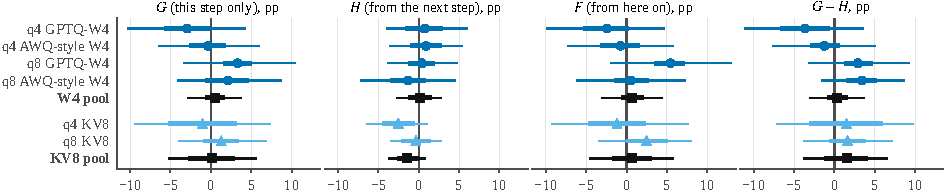
\includegraphics[width=\textwidth]{figures/f2_ghf_forest.pdf}
\caption{Replacement gains $G$, $H$, $F$ and $G-H$ per core cell (pp; each cell's Bank P divergent states). Thick: fixed-pool 95\% (block bootstrap, 20--22 blocks); thin: new-task 95\% (crossed task$\times$block). Squares: equal-weight pools. Within a row, contrasts are paired; between rows, descriptive. Stress cells, $F-G$, $F-H$ and $(\DQ,\DB)$ summaries: Table~\ref{tab:ghf}.} % src: analysis/fork/out/ghf_20261001T211519Z.json; analysis/fork/out/ghf_20261001T211519Z.md
\label{fig:ghf}
\end{figure*}

\paragraph{On average over W4 cells, no option has a detectable gain.} Pooled over the four W4 cells (Figure~\ref{fig:ghf}), $G=+0.5$, $H=+0.2$ and $F=+0.7$\pp{}, and every interval covers zero, as do their differences. % src: analysis/fork/out/ghf_20261001T211519Z.md (pools)

\paragraph{Within cells, the paired gains differ.} In q8 GPTQ-W4, $G=+3.3$ [$+1.6$, $+5.0$]\pp{} exceeds $H=+0.4$ ($G-H=+2.9$ [$+1.3$, $+4.7$]), and $F=+5.4$ exceeds $G$ ($F-G=+2.1$ [$+0.2$, $+4.0$]). In q8 AWQ-W4, $G-H=+3.4$ [$+1.5$, $+5.2$] and $F-G=-1.5$ [$-4.2$, $+0.8$]. In q4 GPTQ-W4, $G=-2.9$ and $G-H=-3.6$ [$-6.6$, $-0.6$]. In the stress cell q8 RTN-W3 (three blocks), $H=+15.3$ and $F=+18.4$ against $G=-0.4$ ($G-H=-15.7$ [$-27.5$, $-3.9$]). In q4 KV8, B continuing after Q's action lowers success ($H=-2.5$ [$-4.5$, $-0.5$], unadjusted). % src: analysis/fork/out/ghf_20261001T211519Z.md (§1; n_tasks)
After Holm adjustment over the four core W4 cells, $G-H$ stays below .05 in both q8 cells ($p=.013$, $.012$) but not in q4 GPTQ-W4 ($p=.069$). % src: analysis/fork/out/ghf_multiplicity_20261001T225727Z.md
These within-cell orderings are exploratory: they hold on the fixed 85 tasks but are not confirmed on new tasks (Table~\ref{tab:ghf-crossed}) or under a second simulator (Appendix~\ref{app:simctrlpmain}), and cells select different states. % src: analysis/fork/out/ghf_20261001T211519Z.md (§1; n_tasks)

\paragraph{A BF16 reference action can lower success.} In q4 GPTQ-W4, B's action lowers success under Q's continuation on the fixed task pool ($G=-2.9$ [$-5.7$, $-0.2$]\pp{}, unadjusted; the new-task interval covers zero), with a similar point estimate under B's ($\DB=-3.2$ [$-6.4$, $+0.2$]). % src: analysis/fork/out/ghf_20261001T211519Z.md (§1, F - H)

\subsection{Continuation dependence per cell and environment}

\begin{figure}[t]
\centering
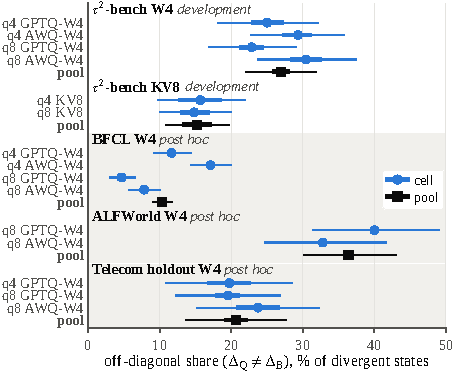
\includegraphics[width=\columnwidth]{figures/f1_controller_dependence.pdf}
\caption{Same action, different value: per-cell share of divergent states with $\DQ\neq\DB$. Thick: fixed-pool 95\% (development: block bootstrap; holdout: block $t$); thin: new-task 95\% (crossed; BFCL/ALFWorld: item bootstrap). Pools: equal weight (holdout: pre-registered weights). Shaded groups are post hoc. Cross-cell comparisons are descriptive.} % src: analysis/fork/out/ghf_20261001T211519Z.json; analysis/fork/out/ext_r2_20261002T024433Z.json; analysis/fork/out/holdout_r2_posthoc_20261002T024414Z.json
\label{fig:ctrl}
\end{figure}

Figure~\ref{fig:ctrl} gives the off-diagonal share per cell; the pooled $(\DQ,\DB)$ tables are in Figure~\ref{fig:3x3}. Because replay is exact, each off-diagonal state shows a real interaction on the success scale, not replay noise. Cohen's $\kappa$ between $\DQ$ and $\DB$, against a marginal-preserving re-pairing of states, is 0.29 in the W4 pool; it measures how well the two effects agree across states, not whether the interaction is significant (Appendix~\ref{app:agreement}). % src: analysis/fork/out/agreement_control_20261002T024240Z.md (§2 equal-weight pools W4:all)
Strict sign reversals are 1.2--4.2\% of states in each W4 and KV8 cell, or 8--14\% of the off-diagonal mass. % src: analysis/fork/out/ghf_20261001T211519Z.md (TL;DR; §2)
In BFCL multi-turn and ALFWorld (post hoc; one run per item; Table~\ref{tab:extr2}), the off-diagonal share is 4.7--17.1\% in the four BFCL W4 cells (pool 10.3\%) and 32.8--40.0\% in the two q8 ALFWorld W4 cells (pool 36.4\%). Continuation dependence therefore does not require an LLM user simulator, and its size differs by environment. % src: analysis/fork/out/ext_r2_20261002T024433Z.md (§3, §6)
The net replacement gain on these benchmarks covers zero except for BFCL q4 AWQ-W4, where it is $-3.8$ [$-6.5$, $-1.3$]\pp{}. % src: analysis/fork/out/ext_20261001T135106Z.md
The value of a fixed replacement policy is $E[G]$, $E[H]$ or $E[F]$, not $E[I]$. All 16 outcome patterns are in Appendix~\ref{app:patterns}.

\subsection{Telecom: development tasks and the holdout's four branches}
\label{app:holdoutdev}

The holdout protocol, its exclusions and strata are in Appendix~\ref{app:prereg}; all 12 blocks were complete, and 1200 of the 1224 units were analysed after 2 structural task$\times$cell exclusions. The cells were q4 GPTQ-W4, q8 GPTQ-W4 and q8 AWQ-W4, weighted 1/2, 1/4, 1/4; the block-$t$ 90\% interval of the primary endpoint is [$-6.08$, $-3.05$]. % src: docs/insights/PREREG_FORK_CONFIRM.md §0; analysis/fork/out/holdout_confirm_20261002T012353Z.md; derived: 1224=34*12*3; 1200=34*12*3-2*12
On 80 telecom development tasks (6 blocks; fixed-pool 95\%), the two q8 holdout cells give $\Gall=+2.7$ [$-4.7$, $+10.1$] (GPTQ-W4) and $-0.6$ [$-4.9$, $+3.7$]\pp{} (AWQ-W4), against $-5.6$ and $-6.6$ on the holdout; q4 has no telecom development forks. % src: analysis/fork/out/dev_all_20261001T093944Z.md (Telecom development); analysis/fork/out/dev_all_20261001T093944Z.json (telecom_cells, t_ci95); analysis/fork/out/holdout_confirm_20261002T012353Z.md (per-cell G)
A post hoc four-branch analysis of the 1180 holdout divergent states (Table~\ref{tab:holdoutr2}) gives $G=-4.6$ [$-7.8$, $-1.5$], $H=-2.8$ [$-6.3$, $+0.6$], $F=-2.5$ [$-6.2$, $+1.3$], $G-H=-1.8$ [$-4.8$, $+1.1$] and mean $I=-5.0$ [$-9.6$, $-0.4$]\pp{} (crossed 95\%), unlike the near-zero development W4 pool, with 20.7\% of states off the diagonal (Figure~\ref{fig:ctrl}). % src: analysis/fork/out/holdout_r2_posthoc_20261002T024414Z.md (§1, §3 pool)
This $G$ conditions on divergence and nearly equals $\Gall$ because 1180 of 1200 units diverge. % src: analysis/fork/out/holdout_r2_posthoc_20261002T024414Z.md (§6); analysis/fork/out/holdout_confirm_20261002T012353Z.md; derived: 1200=396+408+396
In an exploratory analysis of the development data, the top 20\% of tasks hold 57--71\% of all flips in the W4 and KV8 cells (Appendix~\ref{app:concentration}). % src: analysis/fork/out/consequence_v2_20261001T070850Z.json (share_of_consequences_in_top20pct_tasks)

\subsection{Ordinary states and the user simulator}
\label{app:ordinary}

\paragraph{Ordinary states turn over less, mostly through text under our simulator.} At ordinary states, replacing Q's action changes the outcome less often than at first tool-structure divergences (a descriptive comparison of different state populations, with no interval on the difference). Over blocks f01--f03 (task-equal; $t$ intervals over block means), $M$ per sub-bank is 7.8--9.0\% for the q4 W4 cells in U1 and U2B, 4.7--9.0\% for the q8 W4 cells and at most 4.7\% for KV8. The net gain lies within $\pm$2.8\pp{} (U1, U2B) and $\pm$5.0\pp{} (U2Q), and every interval covers zero (Appendix~\ref{app:banku}). % src: analysis/fork/out/bank_u_f01_f02_f03_20261002T003037Z.md (§2)
Identical actions never change the outcome, as determinism implies. After deduplication, 150 of the 208 outcome-changing cell$\times$state rows ($\approx$72.1\%) are class (ii), the same tool structure with different text; 26 involve a different tool name, call count or argument (Table~\ref{tab:taxonomy}). % src: analysis/fork/out/bank_u_f01_f02_f03_20261002T003037Z.md (§3); derived: 150=45+28+44+25+10+6-5-3; 208=99+99+18-5-3; 72.1=100*(45+28+44+25+10+6-5-3)/(99+99+18-5-3); 26=1+11+4+9+0+1
The rows are not independent states: the three blocks repeat the same tasks, and each U2B/U2Q state appears once per cell of a model.
This is a \emph{composition share}: per instance, text, tool/argument and act/talk differences flip the outcome in 14.4\%, 18.2\% and 18.9\% of rows. Text dominates because it is common (1045 of 1357 differing rows), not because each text difference matters more. % src: analysis/fork/out/bank_u_f01_f02_f03_20261002T003037Z.md (§3); derived: 14.4=100*(45+28+44+25+10+6-5-3)/(309+202+277+199+63+33-24-14); 1045=309+202+277+199+63+33-24-14; 18.2=100*(1+11+4+9+0+1)/(19+47+24+40+5+11-1-2); 18.9=100*(10+4+3+14+1+0)/(38+33+34+56+4+7-1-2); 1357=309+202+277+199+63+33-24-14+19+47+24+40+5+11-1-2+38+33+34+56+4+7-1-2
Among simple content features, only an above-median length difference between the two texts co-occurs with outcome change (in all four U1/U2B $\times$ model groups); question, confirmation-request and new-entity flags show no consistent association. These are untested regular-expression features. Bank P cannot see these differences by design. % src: analysis/fork/out/bank_u_f01_f02_f03_20261002T003037Z.md (§3 M rate column; §4)

\paragraph{Sensitivity to the user simulator.} Text actions act through the user simulator, and changing the simulator moves $\tau$-bench outcomes by 9--15 points \citep{seshadri2026lost,jain2026userproxybench}. % src: outputs/.drafts/storyline-v7-lit.md (rows 23-24)
We froze a control before running it: the 39 deduplicated class-(ii) flips of block f01 and 39 matched non-flip states. Their BQ and QQ branches were each re-run three times with a different user simulator, Sonnet 5.5, answering through a file relay from Claude Code subagents (reproducibility limits in the Limitations). % src: docs/RESEARCH_LOG.md W90, W91 (manifests/fork/simctrl_v3.json)
Judged by the sign of the replicate mean, only 7 of the 39 flips keep their direction (95\% CI 0.075--0.335). Six reverse, and 26 vanish (15 both succeed, 2 both fail, 9 ties). Among the matched non-flip states, 11 of 39 become flips (0.15--0.45). Replicates of the same arm disagree in 41\% of flip arms and in 21--26\% of control arms. % src: analysis/fork/out/simctrl_20261001T212742Z.md
\textbf{The Bank U text-difference outcome labels did not reproduce reliably under this alternative relay setting.} The control changes three things at once (simulator model, sampling, relay interface), so it cannot say which of them changed the labels.

\paragraph{Sensitivity of the four-branch results.}
\label{app:simctrlpmain}
Before running, we sampled 80 Bank P states without outcome information (20 per W4 cell, stratified by domain and block) and re-ran all four arms five times each with Sonnet 5.5 as the user, one isolated single-request call per user turn (7896 calls; all integrity checks passed). % src: analysis/fork/out/simctrl_p_20261002T015200Z.md; manifests/fork/simctrl_p_v1.json
Per-state arm outcomes track the original single runs (correlation 0.63--0.68). Pooled over cells, $G=-3.0$ [$-10.2$, $+4.8$], $H=+5.5$ [$+0.0$, $+11.2$] and $G-H=-8.5$ [$-14.8$, $-2.8$]\pp{} under Sonnet, against $G-H=-2.5$ [$-11.2$, $+6.2$] on the same states under the original simulator (change $-6.0$ [$-16.2$, $+4.2$]). % src: analysis/fork/out/simctrl_p_20261002T015200Z.md (pool, all batches)
With 20 states per cell, this control cannot resolve the few-pp contrasts of Table~\ref{tab:ghf} (on this sample even the original simulator gives $G-H=0.0$ in both q8 W4 cells), so it neither confirms nor reverses the within-cell orderings. % src: analysis/fork/out/simctrl_p_20261002T015200Z.md (q8 cells)
Per-cell estimates under both simulators are in Figure~\ref{fig:simctrlp}, and an exploratory mean squared interaction under Sonnet is in Appendix~\ref{app:simctrlp}.

\paragraph{Bank P and Bank U measure different quantities.} Bank P skips text-only differences by design, yet these make up 150 of the 208 outcome-changing rows at ordinary states, and their labels did not reproduce under a second simulator (Appendix~\ref{app:banku}; \S\ref{sec:value}). Including text actions requires a simulator control before their consequences are reported as a property of the action. % src: analysis/fork/out/bank_u_f01_f02_f03_20261002T003037Z.md (§3); analysis/fork/out/simctrl_20261001T212742Z.md; derived: 150=45+28+44+25+10+6-5-3; 208=99+99+18-5-3

\subsection{Token-level analysis}
\label{app:token}

Following \citet{lotfi2026quantized}, we scored every Bank U f01 state at the token level (1140 cell $\times$ state rows, 58 flips), teacher-forcing both models on the generated ids of $a_{\mathrm{B}}$ and $a_{\mathrm{Q}}$. We record truncated top-20 entropy, the top-1 margin and a top-20-union KL, not full entropy or KL. All analyses are exploratory, and f01 is development data. % src: analysis/fork/out/token_mech_20261001T185031Z.md (§0); docs/RESEARCH_LOG.md W88

\paragraph{Uncertainty is associated with divergence.} Q's entropy at the start of its action separates states where B and Q act differently from states where they act identically, with AUC 0.66--0.91 per sub-bank and model. Over all ordinary states, flips also sit at lower Q margins (U1: AUC 0.31 [0.22, 0.40] for q4, 0.24 [0.13, 0.36] for q8; stratified). % src: analysis/fork/out/token_mech_20261001T185031Z.md (§1a, §1b "differing vs exact"); docs/RESEARCH_LOG.md W88

\paragraph{Among divergent states, it does not reliably identify consequences.} Restricting to states where the actions differ removes the ``any difference at all'' signal. In U1 the signal is not detectable: no Q-visible statistic has an interval excluding 0.5 (21 and 9 flips; f01). Only small sub-banks keep a signal: q4 U2B (mean entropy over $a_{\mathrm{Q}}$, AUC 0.73 [0.53, 0.89]) and q4 U2Q (entropy and margin at the action start, AUC 0.90 and 0.10; 10 states, 4 flips). At the first divergent token, pooled entropy and KL do not separate flips from non-flips except in q4 U2Q (KL AUC 0.80 [0.65, 0.93], entropy 0.25 [0.07, 0.48]; 4 flips). Per cell, two further unadjusted intervals exclude 0.5, in opposite directions (U1 q4 GPTQ-W4 entropy 0.30; U2B q4 KV8 KL 0.10). No class of first divergent token reproduces the marker enrichment of \citet{lotfi2026quantized}. The largest q4 enrichment is ordinary word choice (rate ratio 1.89, Fisher $p=.019$, not corrected). % src: analysis/fork/out/token_mech_20261001T185031Z.md (§1a differing_only, §1b, §2); docs/RESEARCH_LOG.md W88
On development data, uncertainty is associated with \emph{where} quantization changes the action more strongly than with \emph{which} changes matter. The frozen trigger of \S\ref{sec:r4} uses held-out blocks f02/f03 (1020 U1 rows). % src: analysis/fork/out/token_mech_20261002T003130Z.md (§3 Validation, U1 S_mm PRIMARY)

\subsection{Same-precision reference per cell}
\label{app:sameprec}

Per model (interim, \pending{$K=6$}), the turnover difference is $\Delta M=+0.6$ [$-3.1$, $+4.3$]\pp{} in q4 and $-2.5$ [$-5.6$, $+0.5$] in q8 (fixed pool, 95\%), with crossed intervals [$-5.5$, $+6.9$] and [$-7.3$, $+2.7$]. Within $\pm$3\pp{}, equivalence is shown for no per-model $\Delta M$ or $\Delta\Gall$; the q8 off-diagonal difference ($+0.40$, 90\% [$-2.12$, $+2.92$]) is the only per-model contrast inside the margin. The protocol originally mapped ``interval includes 0 and $|\Delta M|\le3$\pp{}'' to ``similar''; after the interim result had been seen, an amendment replaced that reading by two one-sided tests, which are stricter, and changed no estimate. % src: analysis/fork/out/sameprec_20261002T142834Z.md (Paired differences; Amendment A1 table; analysis set K = 6); docs/insights/SAMEPREC_PROTOCOL.md (Amendment A1)
Acceptance: every state in both designs passed Q replay and every branch passed the prefix and environment checks; QQ no-op samples passed 265/265 (precision) and 162/162 (same precision), and no directory was quarantined. At the unit level, $\kappa$ is 0.43 in q4 and 0.61 in q8; at the task level, cross-design agreement at matched noise is 0.765 of within-design replication. % src: analysis/fork/out/sameprec_20261002T142834Z.md (Acceptance); analysis/fork/out/sameprec_overlap_20261002T143218Z.md (Agreement; Task-level, pooled cross/within)

W3 stress check (\S\ref{sec:sameprec}; $K=3$): every state passed Q replay, QQ no-op samples passed 31/31 and 39/39, and no directory was quarantined. All branches passed the prefix and environment checks except one of 774 in q8 same precision: a Q$'$Q$'$ branch that ended in an agent-side context overflow, for which the harness records no prefix comparison; its environment hash and first replayed prompt match the frozen state, and by the protocol it counts as a failure, not an exclusion. % src: analysis/fork/out/sameprec_w3_20261003T023933Z.md (Acceptance); analysis/fork/out/sameprec_prefix_check_20261003T030004Z.md


\paragraph{Equivalence tests (W4).} The difference in turnover is $\Delta M=M-M'=-0.98$\pp{} (90\% CI [$-3.26$, $+1.30]$). No precision-specific excess was detected, but equivalence within $\pm$3\pp{} is not shown either (two one-sided tests, $p=0.067$), and the same holds for the net gain ($\Delta\Gall=-1.57$ [$-5.17$, $+2.04$], $p=0.230$) and, descriptively, for the off-diagonal share ($-1.210$ [$-4.09$, $+1.67$], $p=0.133$, as the mean of per-block ratios, which the interval and test use; $-1.216$ as the ratio of block sums). % src: analysis/fork/out/sameprec_20261002T142834Z.md (Amendment A1 table, pool rows); analysis/fork/out/sameprec_20261003T023857Z.json (tost_a1.consistency.d_offdiag: -1.21 stored at 3-decimal rounding); derived: 1.210=1.21

\paragraph{Full substitution (W4).} Under full substitution B flips more units than Q$'$ (193 vs.\ 149; $+4.3$ [$+0.4$, $+8.3$]\pp{}, one of several contrasts); the net difference comes only from substitution-specific units and is not resolved ($\Delta G=-1.6$ [$-6.2$, $+3.0$]\pp{}). Only value measures on the same units reveal this structure. % src: analysis/fork/out/sameprec_split_20261002T145148Z.md (§3 net decomposition; cross-direction counts)

\paragraph{W3 stress pair.} The protocol's complete W3 panel (Q GPTQ-W3, Q$'$ a second W3 calibration draw; q4 and q8, $K=3$ blocks q3--q5, 510 units) is reported next to W4, never pooled with it. The same-precision substitution produces 17.3\pp{} of turnover, the BF16 substitution 18.8\pp{}; off-diagonal shares are 27.6\% and 27.3\%. % src: analysis/fork/out/sameprec_w3_20261003T023933Z.md (TL;DR; Full pool, pool rows); analysis/fork/out/sameprec_w3_split_20261003T024007Z.md (510 units); docs/insights/SAMEPREC_W3_PROTOCOL_20261002.md (K = 3, q3-q5)
$\Delta M=+1.6$\pp{} (95\% [$-0.66$, $+3.80$]) is unresolved: the preregistered $\pm$3\pp{} equivalence test fails ($p=0.055$); that the 90\% interval lies just above zero does not change this. $\Delta\Gall$ is equivalent within $\pm$3\pp{} only in the preregistered pooled population ($+1.2$, $p=0.017$); per model it is $+3.1$ (q4) and $-0.8$\pp{} (q8). The off-diagonal difference is $-0.288$ (ratio of block sums) or $-0.307$ (mean of per-block ratios, used by the interval and test: 90\% [$-11.0$, $+10.4]$, $p=0.27$). % src: analysis/fork/out/sameprec_w3_20261003T023933Z.md (Amendment A1 table; Paired differences); analysis/fork/out/sameprec_w3_20261003T023933Z.json (pooled.paired.dM.ci95; tost_a1.consistency.d_offdiag)
On the action side ($G$), rescued and harmed task$\times$block units overlap ($\kappa=0.60$, $0.68$); the designs may first diverge at different decisions, so this is unit overlap, not a same-state replication. Of 122 units whose $G$ outcome flips, 62 flip under both substitutions, 34 only under BF16 and 26 only under the other W3 checkpoint: 49\% respond to only one. Flip volume, affected units and net upgrade value must be measured separately. % src: analysis/fork/out/sameprec_w3_split_20261003T024007Z.md (Figure-panel table, G rows; TL;DR); derived: 122=62+34+26

\paragraph{Net values on the same-precision blocks.} The reference changes how B's consequences are read, not what they are: on 20 blocks B's action is worth $\Gall=+2.9$\pp{} in q8 and $-1.9$\pp{} in q4 GPTQ-W4 (\S\ref{sec:value}). On the interim same-precision blocks, B's and Q$'$'s net gains ($-0.7$ [$-3.9$, $+2.5$] and $+0.9$ [$-3.1$, $+4.8$]\pp{}) are no conclusion about value; the next comparison asks it directly. % src: analysis/fork/out/dev_all_20261001T070326Z.md; analysis/fork/out/sameprec_20261002T142834Z.md (Full pool, pool q4+q8 rows)

\paragraph{Common-state comparison: details.} Above, each design selects its own divergent states. A pre-registered comparison removes that difference: on 510 ordinary q8 states (85 tasks $\times$ 6 blocks, sampled by a fixed rule), the current action comes from B, from Q (GPTQ-W4, first checkpoint) or from Q$'$ (second checkpoint), and B or Q continues. $K(c)=V(\mathrm{B},c)-V(\mathrm{Q}',c)$ asks what B's action adds beyond another W4 action. A frozen rule claims value only if both intervals exclude zero (Holm), equivalence only if both lie within $\pm$3\pp{} (two one-sided tests). % src: docs/insights/COMMONSTATE_SOURCES_PROTOCOL.md (§2 design, §5 estimands, §6 frozen reading; A1.1); analysis/fork/out/commonstate_q8ext_20261003T231159Z.md (header); derived: 510=85*6
The design first ran three blocks, and that first look was unresolved (under Q's continuation $K=-0.4$\pp{}, 95\%: $t$ [$-9.3$, $+8.5$], bootstrap [$-3.5$, $+2.7$]; under B's $+2.4$\pp{}, [$-3.5$, $+8.2$], [$-0.8$, $+5.5$]). Three more blocks were then added. That decision followed the unresolved first look, so a dated amendment fixed the extension before any new outcome existed, and a two-look sensitivity analysis (Pocock levels from a normal approximation: about 97\% intervals for a difference and 94\% for equivalence) is reported next to the ordinary intervals. The Pocock constant is not calibrated for small-$k$ $t$ intervals, the task bootstrap or the joint rule, so it is a sensitivity analysis, not an exact error guarantee. % src: analysis/fork/out/commonstate_20261002T201612Z.md (Key estimand table); docs/insights/COMMONSTATE_SOURCES_PROTOCOL.md (A1 'What was known', A1.3, D2.2)
After the fixed extension (six blocks), B's action is not shown to be worth more than Q$'$'s, and equivalence is not established. Under Q's continuation, $K=+1.0$\pp{} (95\%: $t$ [$-3.5$, $+5.4$], bootstrap [$-1.2$, $+3.1$]; two-look 97\%: [$-4.2$, $+6.2$], [$-1.4$, $+3.5$]). Under B's, $K=+0.8$\pp{} (95\%: [$-1.8$, $+3.3$] for both; two-look 97\%: [$-2.2$, $+3.8$], [$-2.0$, $+3.7$]). For equivalence under B's continuation, the ordinary 90\% intervals lie within $\pm$3\pp{} ($t$ [$-1.2$, $+2.8$], bootstrap [$-1.4$, $+2.9$]) and the two-look 94\% intervals do not ($t$ [$-1.6$, $+3.2$]); because the extension followed the first look, we do not claim equivalence. Without the 26 states at which earlier studies had already produced outcomes, $K$ is $+0.5$ and $+0.8$\pp{}, also not resolved. % src: analysis/fork/out/commonstate_q8ext_20261003T231159Z.md (Key estimand table; Two-look reading table; Sensitivity without the D2.1 states); docs/insights/COMMONSTATE_SOURCES_PROTOCOL.md (D2.1)
Under Q's continuation, B's action flips $M=7.1$\% of outcomes (rescue 4.1, damage 2.9) for a net $\Delta=+1.2$\pp{} (95\%: $t$ [$-1.3$, $+3.6$]); Q$'$'s flips 8.0\% (4.1, 3.9) for $+0.2$\pp{} ([$-2.3$, $+2.7$]; within $\pm$3\pp{} by two one-sided tests). A second W4 checkpoint's action departs from Q's at least as often as B's does (agreement with Q's action 53.9\% against 55.7\%; B with Q$'$ 57.3\%; Figure~\ref{fig:commonstate}c). The interaction of $K$ with the continuation is $-0.2$\pp{} (95\%: $t$ [$-4.5$, $+4.1$], bootstrap [$-2.7$, $+2.4$]; secondary, not resolved). % src: analysis/fork/out/commonstate_q8ext_20261003T231159Z.md (Contrasts table, c = d1 rows; Action agreement; Interaction table, bf16 − d2 row)
Changing outcomes is thus not improving them; this does not make precision irrelevant or the two actions equivalent.

\begin{figure*}[t]
\centering
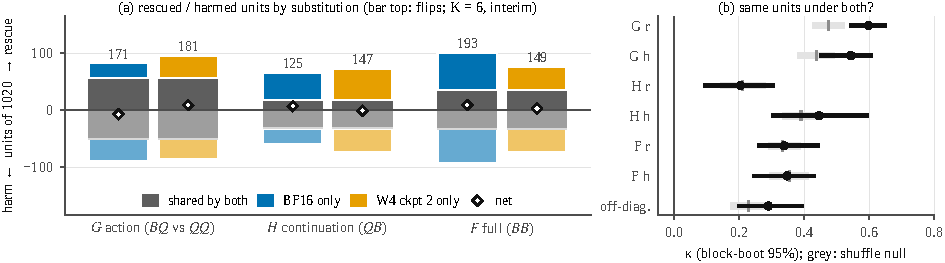
\includegraphics[width=\textwidth]{figures/f7_sameprec_split.pdf}
\caption{Which units the two substitutions rescue and harm (q4 and q8 GPTQ-W4 pooled; 1020 units; interim, \pending{$K=6$}; descriptive). (a)~Per contrast ($G$: action side, BQ vs.\ QQ; $H$: continuation side, QB vs.\ QQ; $F$: full substitution, BB vs.\ QQ) and substitution (B, or the second W4 checkpoint in the B role): rescues above zero and harms below, split into units shared by both substitutions and substitution-specific units; the bar-top number is the flip count and the diamond the net. (b)~Cohen's $\kappa$ of each set between the two substitutions (block-bootstrap 95\%) against a shuffle null (grey: within task and QQ outcome for rescue and harm sets, within task for the off-diagonal set). Rescue under one substitution and harm under the other cannot co-occur, because the QQ episode is shared.} % src: analysis/fork/out/sameprec_split_20261002T145148Z.json; analysis/fork/out/sameprec_split_20261002T145148Z.md
\label{fig:split}
\end{figure*}
